\documentclass[10pt]{article}
\usepackage[a4paper,margin=2.2cm]{geometry}
\usepackage{amsmath,amssymb,booktabs,longtable,graphicx,xcolor,array}
\usepackage{lscape}
\usepackage[hidelinks]{hyperref}
\setlength{\parskip}{0.45em}\setlength{\parindent}{0pt}
\newcommand{\E}{\mathbb{E}}
\newcommand{\RPS}{\mathrm{RPS}}
\newcommand{\CE}{\mathrm{CE}}
\newcommand{\TVD}{\mathrm{TVD}}
\newcommand{\corr}{\mathrm{corr}}
\title{Experiment 26: five new frontier judges, CE-trained versus Pearson-trained calibration at small training sizes\\[0.3em]\large Method, derivation and results \quad (11-23-2026)}
\author{ub9sc for Brando Miranda \quad project: judges-dont-need-psychometrics-or-corr}
\date{11-23-2026 \quad (as of 11-23-2026)}
\begin{document}
\maketitle

\section*{1. What this result does and does not show}
\fbox{\parbox{0.96\linewidth}{
\textbf{Shows.} On one real corpus (160 short answers to 10 homework assignments, each graded 0--5 by two graders), five frontier judges (closed: GPT-6 Astra, Claude Opus 5.5; open weights: Kimi K3, GLM 5.3, DeepSeek V4.1 Flash) were asked once per answer for a probability over the six grades. A calibration of each judge's probabilities was then \emph{chosen from a fixed family of 27 transforms} using only a small number of human ratings, in two ways: by minimising cross-entropy (\textbf{CE fit}) or by maximising Pearson correlation (\textbf{Pearson fit}). On held-out assignments the CE fit had lower ranked probability score (RPS) than the Pearson fit in \textbf{35 of 35} judge-by-budget cells (point estimates). It passed the pre-registered descending significance rule for GPT-6 Astra and Kimi K3 (256 down to 8 training ratings), and \emph{not} for Claude Opus 5.5, GLM 5.3 and DeepSeek V4.1 Flash, which already fail at 256 ratings.\\[0.4em]
\textbf{Does not show.} (i) Not that CE wins everywhere: with only 4 training ratings the CE fit is not significantly better than the Pearson fit in RPS for four of the five judges (DeepSeek is the exception), the CE fit has a \emph{higher} held-out CE than the Pearson fit for GPT-6 Astra (interval excludes 0), and Pearson has lower TVD than CE for Claude Opus 5.5 at 256 and 128 ratings (Table~4). (ii) Not a statement about trained judges in general: only a 27-transform calibration of a frozen judge was fitted, on one course, two graders, ten dependent folds, one judge run per model. (iii) Nothing about VeriBench: fresh VeriBench ratings do not yet exist.\\[0.4em]
\textbf{Why correlation is limited (stated up front).} The Pearson objective sees a judge only through its predicted mean grade $m_i=\sum_g g\,q_{ig}$ for each answer $i$, and only up to level and scale:
\[
\boxed{\;\rho(m,\bar y)=\frac{\sum_i (m_i-\bar m)(\bar y_i-\bar{\bar y})}{\sqrt{\sum_i (m_i-\bar m)^2}\sqrt{\sum_i(\bar y_i-\bar{\bar y})^2}},\qquad \rho(a+b\,m,\bar y)=\rho(m,\bar y)\ \ (b>0)\;}
\]
so it is blind to the spread and shape of $q_i$ (second and higher moments) and to the mean's level and scale. Proper scores (CE, RPS) are minimised only at the full human distribution, which fixes the mean \emph{and} every higher moment. That is the infinite-data statement; whether it helps at small $N$ is exactly what this experiment tests (Section~4).
}}

\section*{2. Data, judges and notation}
\begin{tabular}{p{2.6cm}p{12.4cm}}
\toprule symbol & meaning \\ \midrule
$i$ & an answer (160 in total); $a(i)$ its assignment (10 assignments, 16 answers each) \\
$g\in\{0,\dots,5\}$ & grade \\
$r_{i1},r_{i2}$ & the two graders' grades for answer $i$; $\bar y_i=(r_{i1}+r_{i2})/2$ \\
$H_i\in\Delta^5$ & the human distribution of answer $i$: $H_{ig}=\tfrac12\sum_{j=1}^2\mathbf 1[r_{ij}=g]$ \\
$p_i\in\Delta^5$ & the judge's reported probabilities for answer $i$ (one call, parsed; invalid output becomes uniform) \\
$\theta=(t,b,c)$ & one of 27 calibration settings: $t\in\{0.5,1,2\}$, $b,c\in\{-1,0,1\}$ \\
$q^{\theta}_i$ & calibrated distribution, defined below \\
$m^\theta_i$ & its mean grade $\sum_g g\,q^\theta_{ig}$ \\
$B$ & training budget in individual ratings (4, 8, \dots, 256); in the primary condition $n=B/2$ distinct answers, both graders' ratings \\
\bottomrule
\end{tabular}

Calibration. With smoothing $\tilde p_{ig}=(1-6\cdot10^{-6})p_{ig}+10^{-6}$ and $u_g=(g-2.5)/2.5$,
\[
\boxed{\,q^{\theta}_{ig}=\frac{\exp\!\big(t\log\tilde p_{ig}+b\,u_g+c\,u_g^2\big)}{\sum_{h}\exp\!\big(t\log\tilde p_{ih}+b\,u_h+c\,u_h^2\big)}\,}
\]
$\theta=(1,0,0)$ is the uncalibrated judge. The 27 settings are ordered by distance to this identity.

\section*{3. Derivations}
\subsection*{3.1 The two fits}
Given a training sample $T$ of $n$ answers with ratings $r_{ij}$ ($j=1..k$, $k=2$ primary, $k=1$ secondary):
\begin{align}
\hat\theta_{\CE}&=\arg\min_\theta\ \frac{1}{nk}\sum_{i\in T}\sum_{j=1}^{k}-\log q^\theta_{i,r_{ij}} &&\text{mean individual-rating CE},\\
\hat\theta_{P}&=\arg\max_\theta\ \rho\big(m^\theta_T,\bar y_T\big) &&\text{Pearson of predicted mean vs observed mean grade.}
\end{align}
Ties go to the earliest setting in the identity-ordered grid (within $10^{-12}$). If $\rho$ is undefined for every $\theta$ (no variance), the Pearson fit returns the identity.

\subsection*{3.2 Why Pearson only sees the mean}
$\rho$ depends on $\theta$ only through the vector $(m^\theta_i)_{i\in T}$. If two settings give $m^{\theta'}_i=a+b\,m^\theta_i$ with $b>0$ on $T$, then $\rho$ is identical, because centring removes $a$ and the denominator rescales by $b$. Hence two judges with equal means up to level and scale are indistinguishable to this objective, whatever their predicted spread. Concretely, the temperature $t$ changes spread and mean together, so a Pearson fit can only prefer $t$ through its effect on the means.

\subsection*{3.3 Why CE and RPS are proper, so they see every moment}
For a target distribution $H$ and forecast $q$, $\E_{r\sim H}[-\log q_r]=-\sum_g H_g\log q_g=\mathrm{H}(H)+\mathrm{KL}(H\,\|\,q)\ge \mathrm{H}(H)$, with equality only at $q=H$. For RPS, with $F_k=\sum_{g\le k}q_g$, $G_k=\sum_{g\le k}H_g$ and the observed rating $r\sim H$:
\begin{align}
\E_r\Big[\tfrac15\sum_{k=0}^{4}\big(F_k-\mathbf 1[r\le k]\big)^2\Big]
&=\tfrac15\sum_{k=0}^{4}\Big(F_k^2-2F_k\,\E\mathbf 1[r\le k]+\E\mathbf 1[r\le k]^2\Big)\notag\\
&=\boxed{\tfrac15\sum_{k=0}^{4}\big(F_k^2-2F_kG_k+G_k\big)}=\tfrac15\sum_{k=0}^4\big(F_k-G_k\big)^2+\tfrac15\sum_{k=0}^4 G_k(1-G_k),
\end{align}
using $\mathbf 1^2=\mathbf 1$ and $\E\mathbf 1[r\le k]=G_k$. The last term does not depend on $q$, so the expected RPS is minimised only at $F=G$, i.e.\ $q=H$. The code scores each held-out answer with the formula in the box, using $H_i$ as the distribution of the observed rating.

\subsection*{3.4 Test metrics, comparators and the sign convention}
For a held-out answer $i$ and forecast $q_i$: $\RPS_i$ as above with $G=\mathrm{cdf}(H_i)$; $\CE_i=-\sum_g H_{ig}\log q_{ig}$ (nats); $\TVD_i=\tfrac12\sum_g|q_{ig}-H_{ig}|$. Per fold the metric is the mean over the 16 held-out answers and over 200 seeded training draws (SeedSequence$[20261121,\text{held-out},\text{draw}]$), then the ten fold values are the data. Comparators: the uniform forecast, the identity (uncalibrated judge) and the training histogram with 0.5 pseudo-count per grade.
\[
\boxed{\ \Delta_f(\text{comparator})=\text{metric}_f(\text{comparator})-\text{metric}_f(\text{CE fit}),\ \ f=1,\dots,10\ }\quad\text{positive means the CE fit is better.}
\]

\subsection*{3.5 Interval and the descending rule}
Folds share training answers, so I use the overlap-adjusted standard error
\[
\boxed{\ \mathrm{SE}=s_\Delta\sqrt{\tfrac1{10}+\tfrac19},\qquad \text{95\% interval}=\bar\Delta\pm t_{0.975,9}\,\mathrm{SE}\ }
\]
with $s_\Delta$ the sample standard deviation of the ten $\Delta_f$ and 9 degrees of freedom. Confirmatory rule (frozen before any grade was read): test $B=256,128,\dots,4$ in descending order; a budget passes if the one-sided lower bounds of $\bar\Delta$ against the Pearson fit \emph{and} against uniform are both above 0, at level $\alpha=0.01$ per judge for the five new judges ($\alpha=0.025$ for the two experiment~21 judges); stop formal claims at the first failure. Later budgets are then descriptive only.

\section*{4. Results (primary condition: two ratings per answer; RPS lower is better)}
\textbf{Bottom line.} CE fit beat Pearson fit on RPS at all 35 judge-by-budget cells. The advantage is $0.02$--$0.03$ RPS at mid budgets for four judges (smaller for Claude Opus 5.5), small next to the gap to uniform ($0.15$--$0.19$). The formal rule passes for GPT-6 Astra and Kimi K3 from 256 down to 8 ratings; it fails at 4 ratings for both (Pearson and CE are within noise with two training answers). For Claude Opus 5.5 ($+0.0037$, 95\% interval $[-0.0025,+0.0098]$), GLM 5.3 ($+0.0195$, lower one-sided bound at $\alpha=0.01$ is $-0.0021$) and DeepSeek V4.1 Flash ($+0.0040$, $[-0.0044,+0.0124]$) the rule fails already at 256, so no formal claim is made below that; descriptively their intervals exclude 0 at smaller budgets (Table~2). Against the training histogram the CE fit is better for four judges at every budget and for DeepSeek only at 16 ratings and fewer.

\begin{center}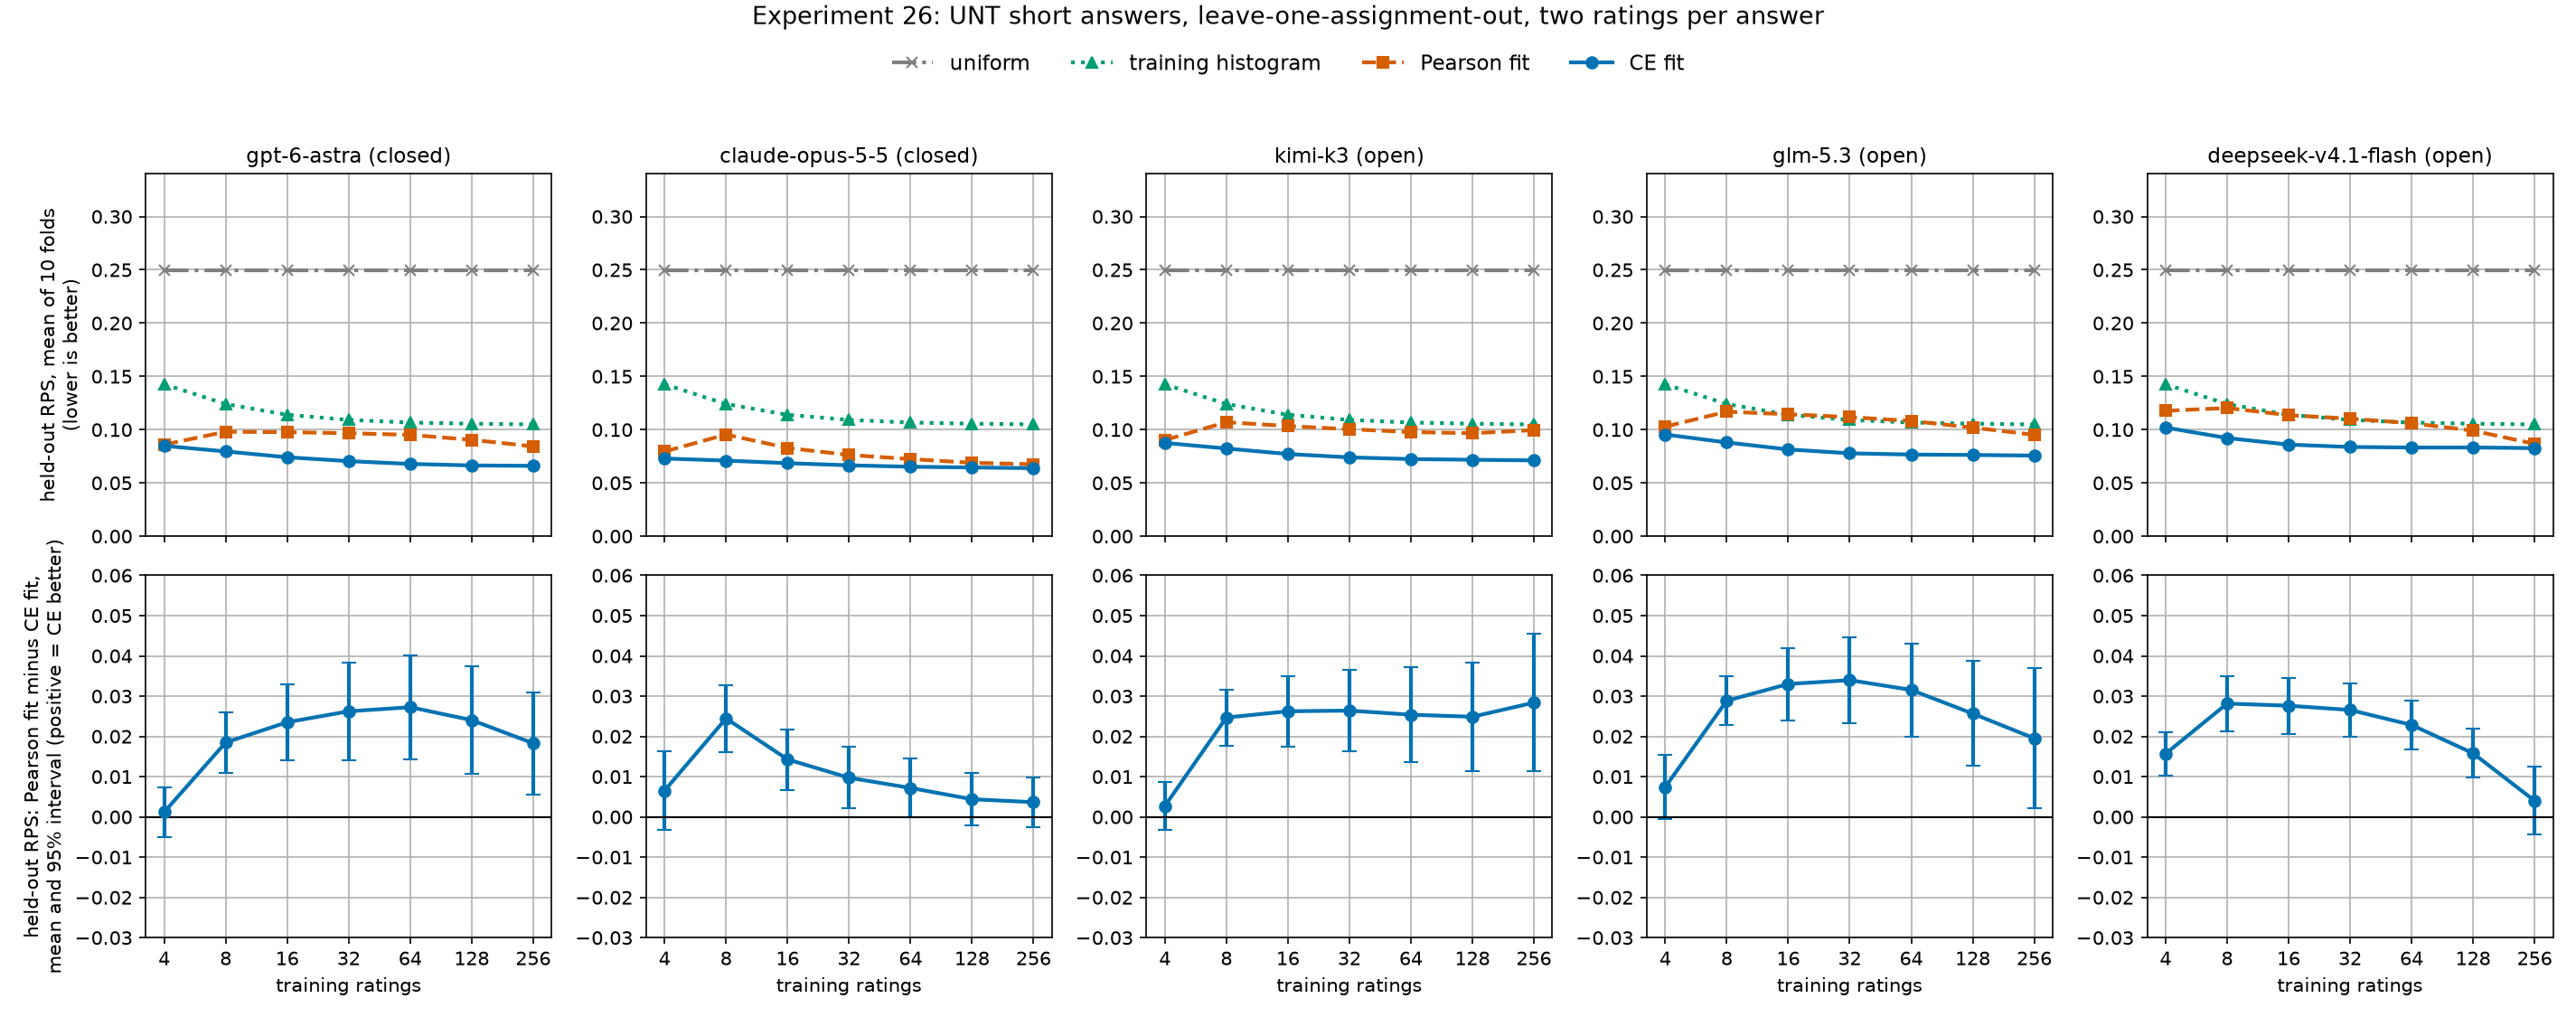
\includegraphics[width=\linewidth]{results/fig_learning_curves_11-23-2026.png}\end{center}
\textit{Figure.} Top: held-out RPS by training ratings. Bottom: Pearson fit minus CE fit with 95\% interval. Grid on; positive means CE better.

\textbf{Pattern.} The advantage is largest at 8--64 ratings and shrinks at 256 for the strongest closed judges (Claude Opus 5.5 and, in experiment~21, Claude Sonnet 5: $+0.0001$ at 256), whose mean grade is already close to the human mean, leaving Pearson little to lose. The uncalibrated judge is as good as or better than the Pearson fit at most budgets (Table~1; for GPT-6 Astra at 8 ratings 0.0858 uncalibrated against 0.0981 Pearson fit), so the Pearson fit adds nothing there and can hurt. The CE fit has lower RPS than the uncalibrated judge in all 35 cells; its 95\% interval against the uncalibrated judge excludes 0 at 256 ratings for all five judges, and at 4 ratings only for DeepSeek.

\textbf{Where Pearson is not beaten} (Table~4): RPS at 4 ratings for four judges (all but DeepSeek); Claude Opus 5.5 at 256, 128 and 64; DeepSeek at 256. In held-out CE and TVD the picture is weaker for CE: at 4 ratings the CE fit has higher CE than the Pearson fit for GPT-6 Astra ($-0.159$, interval $[-0.238,-0.080]$; Kimi K3 and GLM 5.3 also negative, intervals include 0), and Claude Opus 5.5 has lower TVD under Pearson ($-0.0243$ at 256, $-0.0129$ at 128, intervals exclude 0). With two training answers, the minimum-CE transform can be extreme, which hurts held-out CE.

\textbf{Experiment~21 judges re-analysed} (Table~7): Qwen passes at all budgets (advantage $+0.07$ to $+0.12$; its Pearson fit is worse than uniform); Claude Sonnet 5 fails at 256 ($+0.0001$) and is positive at 128 and below, matching Codex's decisions (pass flags and numbers agree; only the status wording differs).

\section*{5. Checks, cost and caveats}
\textbf{Independent check.} A second implementation written for this experiment reproduces experiment~21's Qwen and Claude Sonnet 5 results: 1170 of 1170 score values and 936 of 936 contrast values agree within $3.5\cdot10^{-11}$. A first run disagreed by up to $3\cdot10^{-4}$ in 9 values because the $10^{-12}$ tie tolerance was applied to a summed rather than a mean-per-rating CE; fixed, and the agreement above is after the fix. The author of the second implementation read experiment~21's schedule and selection code first, so it catches transcription errors rather than being a blind rewrite.

\textbf{Cost.} About \$1.34 estimated in total (GPT-6 Astra \$0.90, Claude Opus 5.5 \$0.45; the three open-weight models are listed at \$0 on the gateway), against the \$100 cap and \$80 stop. Table~8.

\textbf{Harness and models.} All judge calls: the Stanford AI API Gateway chat-completions endpoint, one call per answer with the same system and user prompt for every judge, no retries on content. GPT-6 Astra was first tried on the personal Codex plan route but rate-limited (157 of 160 calls failed, none used) and was moved to the gateway (Amendment~1). Claude Opus 5.5 was run through the gateway, not through Claude Code, so it is not the same harness as experiment~21's Claude Sonnet 5. Analysis: ub9sc's Python (numpy/scipy), cross-checked against Codex's experiment~21 code.

\textbf{Caveats.} One course (UNT), two graders, ten folds that share training answers (the interval is adjusted, not exact); each judge ran once, so judge sampling noise is not separated from fold noise; cross-experiment comparisons with experiment~21 mix harnesses; Claude Opus 5.5 produced 4 and GLM 5.3 produced 1 unusable outputs, which became uniform forecasts and stay in the analysis (Table~9); the open-weight costs are \$0 at the gateway's listed rate, not a measured price. Not covered: fresh VeriBench ratings (not yet collected), any judge fine-tuned rather than calibrated, other corpora. The claim ``CE is better even with limited data'' is therefore \emph{supported on this one corpus for RPS from 256 down to 8 ratings by the formal rule for two judges, only descriptively for the other three, and not supported at 4 ratings for four of five judges}; it is not shown in general.

\clearpage
\newgeometry{paperwidth=29.7cm,paperheight=21cm,margin=1.5cm}\pdfpagewidth=29.7cm \pdfpageheight=21cm
\section*{Appendix: tables}
\scriptsize\setlength{\tabcolsep}{2pt}
\textbf{Table 1.} Held-out RPS (lower is better), two ratings per answer, mean of ten folds.\par\begin{longtable}{lrrrrrr}
\toprule
judge & training ratings & CE fit & Pearson fit & uncalibrated & training histogram & uniform \\
\midrule
\endfirsthead
\toprule
judge & training ratings & CE fit & Pearson fit & uncalibrated & training histogram & uniform \\
\midrule
\endhead
gpt-6-astra & 256 & 0.0660 & 0.0843 & 0.0858 & 0.1049 & 0.2497 \\
gpt-6-astra & 128 & 0.0664 & 0.0905 & 0.0858 & 0.1056 & 0.2497 \\
gpt-6-astra & 64 & 0.0678 & 0.0951 & 0.0858 & 0.1067 & 0.2497 \\
gpt-6-astra & 32 & 0.0705 & 0.0967 & 0.0858 & 0.1092 & 0.2497 \\
gpt-6-astra & 16 & 0.0741 & 0.0976 & 0.0858 & 0.1140 & 0.2497 \\
gpt-6-astra & 8 & 0.0796 & 0.0981 & 0.0858 & 0.1241 & 0.2497 \\
gpt-6-astra & 4 & 0.0848 & 0.0860 & 0.0858 & 0.1426 & 0.2497 \\
claude-opus-5-5 & 256 & 0.0639 & 0.0675 & 0.0788 & 0.1049 & 0.2497 \\
claude-opus-5-5 & 128 & 0.0645 & 0.0689 & 0.0788 & 0.1056 & 0.2497 \\
claude-opus-5-5 & 64 & 0.0652 & 0.0724 & 0.0788 & 0.1067 & 0.2497 \\
claude-opus-5-5 & 32 & 0.0666 & 0.0763 & 0.0788 & 0.1092 & 0.2497 \\
claude-opus-5-5 & 16 & 0.0686 & 0.0829 & 0.0788 & 0.1140 & 0.2497 \\
claude-opus-5-5 & 8 & 0.0710 & 0.0954 & 0.0788 & 0.1241 & 0.2497 \\
claude-opus-5-5 & 4 & 0.0729 & 0.0795 & 0.0788 & 0.1426 & 0.2497 \\
kimi-k3 & 256 & 0.0712 & 0.0996 & 0.0899 & 0.1049 & 0.2497 \\
kimi-k3 & 128 & 0.0718 & 0.0966 & 0.0899 & 0.1056 & 0.2497 \\
kimi-k3 & 64 & 0.0724 & 0.0978 & 0.0899 & 0.1067 & 0.2497 \\
kimi-k3 & 32 & 0.0740 & 0.1004 & 0.0899 & 0.1092 & 0.2497 \\
kimi-k3 & 16 & 0.0772 & 0.1034 & 0.0899 & 0.1140 & 0.2497 \\
kimi-k3 & 8 & 0.0823 & 0.1070 & 0.0899 & 0.1241 & 0.2497 \\
kimi-k3 & 4 & 0.0876 & 0.0903 & 0.0899 & 0.1426 & 0.2497 \\
glm-5.3 & 256 & 0.0757 & 0.0952 & 0.1027 & 0.1049 & 0.2497 \\
glm-5.3 & 128 & 0.0763 & 0.1019 & 0.1027 & 0.1056 & 0.2497 \\
glm-5.3 & 64 & 0.0766 & 0.1082 & 0.1027 & 0.1067 & 0.2497 \\
glm-5.3 & 32 & 0.0778 & 0.1118 & 0.1027 & 0.1092 & 0.2497 \\
glm-5.3 & 16 & 0.0815 & 0.1145 & 0.1027 & 0.1140 & 0.2497 \\
glm-5.3 & 8 & 0.0880 & 0.1169 & 0.1027 & 0.1241 & 0.2497 \\
glm-5.3 & 4 & 0.0955 & 0.1029 & 0.1027 & 0.1426 & 0.2497 \\
deepseek-v4.1-flash & 256 & 0.0827 & 0.0867 & 0.1176 & 0.1049 & 0.2497 \\
deepseek-v4.1-flash & 128 & 0.0833 & 0.0991 & 0.1176 & 0.1056 & 0.2497 \\
deepseek-v4.1-flash & 64 & 0.0832 & 0.1061 & 0.1176 & 0.1067 & 0.2497 \\
deepseek-v4.1-flash & 32 & 0.0838 & 0.1103 & 0.1176 & 0.1092 & 0.2497 \\
deepseek-v4.1-flash & 16 & 0.0860 & 0.1136 & 0.1176 & 0.1140 & 0.2497 \\
deepseek-v4.1-flash & 8 & 0.0922 & 0.1203 & 0.1176 & 0.1241 & 0.2497 \\
deepseek-v4.1-flash & 4 & 0.1020 & 0.1177 & 0.1176 & 0.1426 & 0.2497 \\
\bottomrule
\end{longtable}

\textbf{Table 2.} CE-fit advantage in RPS (comparator minus CE fit; positive = CE better), 95\% two-sided interval, and descending formal test (alpha 0.01 per judge). ``not\_tested\_after\_failure'' rows are descriptive only.\par\begin{longtable}{lrrrrrr}
\toprule
judge & training ratings & vs Pearson fit & vs uniform & vs training histogram & folds CE > Pearson & formal status \\
\midrule
\endfirsthead
\toprule
judge & training ratings & vs Pearson fit & vs uniform & vs training histogram & folds CE > Pearson & formal status \\
\midrule
\endhead
gpt-6-astra & 256 & +0.0183 [+0.0056, +0.0310] & +0.1837 [+0.1484, +0.2190] & +0.0389 [+0.0167, +0.0611] & 9/10 & pass \\
gpt-6-astra & 128 & +0.0240 [+0.0108, +0.0373] & +0.1833 [+0.1475, +0.2191] & +0.0392 [+0.0177, +0.0607] & 9/10 & pass \\
gpt-6-astra & 64 & +0.0273 [+0.0144, +0.0401] & +0.1819 [+0.1457, +0.2180] & +0.0388 [+0.0178, +0.0598] & 9/10 & pass \\
gpt-6-astra & 32 & +0.0262 [+0.0141, +0.0383] & +0.1793 [+0.1429, +0.2156] & +0.0387 [+0.0176, +0.0599] & 10/10 & pass \\
gpt-6-astra & 16 & +0.0235 [+0.0140, +0.0330] & +0.1756 [+0.1392, +0.2120] & +0.0399 [+0.0190, +0.0608] & 10/10 & pass \\
gpt-6-astra & 8 & +0.0185 [+0.0110, +0.0260] & +0.1702 [+0.1324, +0.2079] & +0.0445 [+0.0224, +0.0666] & 10/10 & pass \\
gpt-6-astra & 4 & +0.0012 [-0.0050, +0.0074] & +0.1649 [+0.1258, +0.2041] & +0.0578 [+0.0320, +0.0836] & 6/10 & fail \\
claude-opus-5-5 & 256 & +0.0037 [-0.0025, +0.0098] & +0.1859 [+0.1521, +0.2196] & +0.0411 [+0.0184, +0.0637] & 7/10 & fail \\
claude-opus-5-5 & 128 & +0.0044 [-0.0021, +0.0109] & +0.1852 [+0.1501, +0.2203] & +0.0411 [+0.0184, +0.0638] & 9/10 & not\_tested\_after\_failure \\
claude-opus-5-5 & 64 & +0.0072 [-0.0001, +0.0144] & +0.1845 [+0.1492, +0.2198] & +0.0415 [+0.0183, +0.0646] & 9/10 & not\_tested\_after\_failure \\
claude-opus-5-5 & 32 & +0.0097 [+0.0021, +0.0174] & +0.1832 [+0.1483, +0.2180] & +0.0426 [+0.0198, +0.0655] & 9/10 & not\_tested\_after\_failure \\
claude-opus-5-5 & 16 & +0.0143 [+0.0068, +0.0218] & +0.1812 [+0.1471, +0.2152] & +0.0454 [+0.0233, +0.0675] & 10/10 & not\_tested\_after\_failure \\
claude-opus-5-5 & 8 & +0.0245 [+0.0161, +0.0328] & +0.1788 [+0.1452, +0.2123] & +0.0531 [+0.0326, +0.0736] & 10/10 & not\_tested\_after\_failure \\
claude-opus-5-5 & 4 & +0.0065 [-0.0033, +0.0164] & +0.1768 [+0.1438, +0.2098] & +0.0696 [+0.0484, +0.0908] & 8/10 & not\_tested\_after\_failure \\
kimi-k3 & 256 & +0.0284 [+0.0113, +0.0454] & +0.1785 [+0.1389, +0.2182] & +0.0337 [+0.0143, +0.0532] & 9/10 & pass \\
kimi-k3 & 128 & +0.0249 [+0.0114, +0.0383] & +0.1780 [+0.1388, +0.2171] & +0.0338 [+0.0150, +0.0527] & 9/10 & pass \\
kimi-k3 & 64 & +0.0254 [+0.0135, +0.0373] & +0.1773 [+0.1384, +0.2162] & +0.0343 [+0.0158, +0.0528] & 10/10 & pass \\
kimi-k3 & 32 & +0.0264 [+0.0163, +0.0365] & +0.1757 [+0.1367, +0.2147] & +0.0352 [+0.0168, +0.0535] & 10/10 & pass \\
kimi-k3 & 16 & +0.0262 [+0.0175, +0.0350] & +0.1726 [+0.1335, +0.2116] & +0.0368 [+0.0188, +0.0548] & 10/10 & pass \\
kimi-k3 & 8 & +0.0247 [+0.0177, +0.0317] & +0.1674 [+0.1270, +0.2078] & +0.0417 [+0.0219, +0.0616] & 10/10 & pass \\
kimi-k3 & 4 & +0.0027 [-0.0033, +0.0088] & +0.1622 [+0.1207, +0.2036] & +0.0550 [+0.0307, +0.0794] & 8/10 & fail \\
glm-5.3 & 256 & +0.0195 [+0.0022, +0.0369] & +0.1740 [+0.1333, +0.2148] & +0.0292 [+0.0038, +0.0547] & 10/10 & fail \\
glm-5.3 & 128 & +0.0257 [+0.0127, +0.0387] & +0.1734 [+0.1334, +0.2134] & +0.0293 [+0.0043, +0.0543] & 10/10 & not\_tested\_after\_failure \\
glm-5.3 & 64 & +0.0315 [+0.0200, +0.0431] & +0.1731 [+0.1337, +0.2125] & +0.0300 [+0.0056, +0.0545] & 10/10 & not\_tested\_after\_failure \\
glm-5.3 & 32 & +0.0340 [+0.0233, +0.0447] & +0.1719 [+0.1327, +0.2111] & +0.0313 [+0.0079, +0.0548] & 10/10 & not\_tested\_after\_failure \\
glm-5.3 & 16 & +0.0330 [+0.0241, +0.0420] & +0.1683 [+0.1297, +0.2068] & +0.0325 [+0.0098, +0.0552] & 10/10 & not\_tested\_after\_failure \\
glm-5.3 & 8 & +0.0289 [+0.0229, +0.0349] & +0.1617 [+0.1223, +0.2012] & +0.0361 [+0.0127, +0.0594] & 10/10 & not\_tested\_after\_failure \\
glm-5.3 & 4 & +0.0074 [-0.0004, +0.0153] & +0.1543 [+0.1141, +0.1944] & +0.0471 [+0.0207, +0.0736] & 9/10 & not\_tested\_after\_failure \\
deepseek-v4.1-flash & 256 & +0.0040 [-0.0044, +0.0124] & +0.1670 [+0.1242, +0.2098] & +0.0222 [-0.0068, +0.0513] & 6/10 & fail \\
deepseek-v4.1-flash & 128 & +0.0158 [+0.0097, +0.0219] & +0.1664 [+0.1244, +0.2085] & +0.0223 [-0.0062, +0.0508] & 10/10 & not\_tested\_after\_failure \\
deepseek-v4.1-flash & 64 & +0.0229 [+0.0168, +0.0289] & +0.1665 [+0.1250, +0.2080] & +0.0235 [-0.0045, +0.0514] & 10/10 & not\_tested\_after\_failure \\
deepseek-v4.1-flash & 32 & +0.0266 [+0.0200, +0.0332] & +0.1660 [+0.1251, +0.2068] & +0.0254 [-0.0014, +0.0522] & 10/10 & not\_tested\_after\_failure \\
deepseek-v4.1-flash & 16 & +0.0276 [+0.0207, +0.0346] & +0.1637 [+0.1236, +0.2039] & +0.0280 [+0.0022, +0.0538] & 10/10 & not\_tested\_after\_failure \\
deepseek-v4.1-flash & 8 & +0.0282 [+0.0213, +0.0351] & +0.1576 [+0.1169, +0.1982] & +0.0319 [+0.0057, +0.0581] & 10/10 & not\_tested\_after\_failure \\
deepseek-v4.1-flash & 4 & +0.0157 [+0.0103, +0.0210] & +0.1477 [+0.1051, +0.1903] & +0.0406 [+0.0117, +0.0695] & 10/10 & not\_tested\_after\_failure \\
\bottomrule
\end{longtable}

\textbf{Table 3.} Held-out CE (nats) and TVD, two ratings per answer (lower is better).\par\begin{longtable}{lrrrrrrr}
\toprule
judge & training ratings & CE: CE fit & CE: Pearson fit & CE: uniform & TVD: CE fit & TVD: Pearson fit & TVD: uniform \\
\midrule
\endfirsthead
\toprule
judge & training ratings & CE: CE fit & CE: Pearson fit & CE: uniform & TVD: CE fit & TVD: Pearson fit & TVD: uniform \\
\midrule
\endhead
gpt-6-astra & 256 & 0.834 & 0.969 & 1.792 & 0.332 & 0.356 & 0.767 \\
gpt-6-astra & 128 & 0.839 & 1.066 & 1.792 & 0.331 & 0.356 & 0.767 \\
gpt-6-astra & 64 & 0.854 & 1.138 & 1.792 & 0.332 & 0.363 & 0.767 \\
gpt-6-astra & 32 & 0.883 & 1.172 & 1.792 & 0.334 & 0.370 & 0.767 \\
gpt-6-astra & 16 & 0.942 & 1.223 & 1.792 & 0.335 & 0.371 & 0.767 \\
gpt-6-astra & 8 & 1.057 & 1.307 & 1.792 & 0.337 & 0.366 & 0.767 \\
gpt-6-astra & 4 & 1.204 & 1.045 & 1.792 & 0.336 & 0.325 & 0.767 \\
claude-opus-5-5 & 256 & 0.828 & 0.877 & 1.792 & 0.334 & 0.309 & 0.767 \\
claude-opus-5-5 & 128 & 0.836 & 0.885 & 1.792 & 0.325 & 0.312 & 0.767 \\
claude-opus-5-5 & 64 & 0.844 & 0.906 & 1.792 & 0.320 & 0.322 & 0.767 \\
claude-opus-5-5 & 32 & 0.855 & 0.930 & 1.792 & 0.320 & 0.334 & 0.767 \\
claude-opus-5-5 & 16 & 0.875 & 0.971 & 1.792 & 0.324 & 0.356 & 0.767 \\
claude-opus-5-5 & 8 & 0.898 & 1.037 & 1.792 & 0.330 & 0.391 & 0.767 \\
claude-opus-5-5 & 4 & 0.918 & 0.928 & 1.792 & 0.333 & 0.402 & 0.767 \\
kimi-k3 & 256 & 0.966 & 1.879 & 1.792 & 0.352 & 0.378 & 0.767 \\
kimi-k3 & 128 & 0.973 & 1.622 & 1.792 & 0.356 & 0.381 & 0.767 \\
kimi-k3 & 64 & 0.993 & 1.509 & 1.792 & 0.359 & 0.393 & 0.767 \\
kimi-k3 & 32 & 1.040 & 1.499 & 1.792 & 0.360 & 0.407 & 0.767 \\
kimi-k3 & 16 & 1.128 & 1.524 & 1.792 & 0.360 & 0.416 & 0.767 \\
kimi-k3 & 8 & 1.281 & 1.604 & 1.792 & 0.362 & 0.419 & 0.767 \\
kimi-k3 & 4 & 1.446 & 1.307 & 1.792 & 0.363 & 0.390 & 0.767 \\
glm-5.3 & 256 & 1.027 & 1.337 & 1.792 & 0.355 & 0.421 & 0.767 \\
glm-5.3 & 128 & 1.033 & 1.482 & 1.792 & 0.361 & 0.426 & 0.767 \\
glm-5.3 & 64 & 1.041 & 1.553 & 1.792 & 0.365 & 0.429 & 0.767 \\
glm-5.3 & 32 & 1.067 & 1.601 & 1.792 & 0.368 & 0.432 & 0.767 \\
glm-5.3 & 16 & 1.154 & 1.668 & 1.792 & 0.372 & 0.434 & 0.767 \\
glm-5.3 & 8 & 1.340 & 1.790 & 1.792 & 0.380 & 0.432 & 0.767 \\
glm-5.3 & 4 & 1.563 & 1.507 & 1.792 & 0.386 & 0.404 & 0.767 \\
deepseek-v4.1-flash & 256 & 1.028 & 1.109 & 1.792 & 0.337 & 0.360 & 0.767 \\
deepseek-v4.1-flash & 128 & 1.037 & 1.401 & 1.792 & 0.342 & 0.376 & 0.767 \\
deepseek-v4.1-flash & 64 & 1.039 & 1.556 & 1.792 & 0.345 & 0.388 & 0.767 \\
deepseek-v4.1-flash & 32 & 1.048 & 1.583 & 1.792 & 0.349 & 0.397 & 0.767 \\
deepseek-v4.1-flash & 16 & 1.082 & 1.669 & 1.792 & 0.355 & 0.403 & 0.767 \\
deepseek-v4.1-flash & 8 & 1.242 & 1.921 & 1.792 & 0.365 & 0.412 & 0.767 \\
deepseek-v4.1-flash & 4 & 1.584 & 1.715 & 1.792 & 0.379 & 0.397 & 0.767 \\
\bottomrule
\end{longtable}

\textbf{Table 4.} Every primary-condition case where the Pearson fit is not significantly worse than the CE fit. Advantage = Pearson-fit metric minus CE-fit metric; negative means CE worse.\par\begin{longtable}{lrrrrr}
\toprule
judge & training ratings & metric & Pearson minus CE & 95\% interval & reading \\
\midrule
\endfirsthead
\toprule
judge & training ratings & metric & Pearson minus CE & 95\% interval & reading \\
\midrule
\endhead
gpt-6-astra & 4 & rps & +0.0012 & [-0.0050, +0.0074] & CE fit better on average, interval includes 0 \\
gpt-6-astra & 4 & ce & -0.1592 & [-0.2384, -0.0801] & Pearson fit better on average \\
gpt-6-astra & 4 & tvd & -0.0110 & [-0.0305, +0.0085] & Pearson fit better on average \\
claude-opus-5-5 & 256 & rps & +0.0037 & [-0.0025, +0.0098] & CE fit better on average, interval includes 0 \\
claude-opus-5-5 & 256 & ce & +0.0485 & [-0.0170, +0.1140] & CE fit better on average, interval includes 0 \\
claude-opus-5-5 & 256 & tvd & -0.0243 & [-0.0368, -0.0118] & Pearson fit better on average \\
claude-opus-5-5 & 128 & rps & +0.0044 & [-0.0021, +0.0109] & CE fit better on average, interval includes 0 \\
claude-opus-5-5 & 128 & tvd & -0.0129 & [-0.0219, -0.0038] & Pearson fit better on average \\
claude-opus-5-5 & 64 & rps & +0.0072 & [-0.0001, +0.0144] & CE fit better on average, interval includes 0 \\
claude-opus-5-5 & 64 & tvd & +0.0014 & [-0.0071, +0.0099] & CE fit better on average, interval includes 0 \\
claude-opus-5-5 & 4 & rps & +0.0065 & [-0.0033, +0.0164] & CE fit better on average, interval includes 0 \\
claude-opus-5-5 & 4 & ce & +0.0101 & [-0.0871, +0.1073] & CE fit better on average, interval includes 0 \\
kimi-k3 & 256 & tvd & +0.0257 & [-0.0259, +0.0772] & CE fit better on average, interval includes 0 \\
kimi-k3 & 128 & tvd & +0.0245 & [-0.0116, +0.0607] & CE fit better on average, interval includes 0 \\
kimi-k3 & 4 & rps & +0.0027 & [-0.0033, +0.0088] & CE fit better on average, interval includes 0 \\
kimi-k3 & 4 & ce & -0.1383 & [-0.2937, +0.0172] & Pearson fit better on average \\
glm-5.3 & 4 & rps & +0.0074 & [-0.0004, +0.0153] & CE fit better on average, interval includes 0 \\
glm-5.3 & 4 & ce & -0.0559 & [-0.1551, +0.0433] & Pearson fit better on average \\
deepseek-v4.1-flash & 256 & rps & +0.0040 & [-0.0044, +0.0124] & CE fit better on average, interval includes 0 \\
deepseek-v4.1-flash & 256 & ce & +0.0814 & [-0.0317, +0.1945] & CE fit better on average, interval includes 0 \\
\bottomrule
\end{longtable}

\textbf{Table 5.} CE fit versus the training histogram (descriptive).\par\begin{longtable}{lrrr}
\toprule
judge & training ratings & CE-fit advantage in RPS [95\% interval] & reading \\
\midrule
\endfirsthead
\toprule
judge & training ratings & CE-fit advantage in RPS [95\% interval] & reading \\
\midrule
\endhead
gpt-6-astra & 256 & +0.0389 [+0.0167, +0.0611] & CE fit better \\
gpt-6-astra & 128 & +0.0392 [+0.0177, +0.0607] & CE fit better \\
gpt-6-astra & 64 & +0.0388 [+0.0178, +0.0598] & CE fit better \\
gpt-6-astra & 32 & +0.0387 [+0.0176, +0.0599] & CE fit better \\
gpt-6-astra & 16 & +0.0399 [+0.0190, +0.0608] & CE fit better \\
gpt-6-astra & 8 & +0.0445 [+0.0224, +0.0666] & CE fit better \\
gpt-6-astra & 4 & +0.0578 [+0.0320, +0.0836] & CE fit better \\
claude-opus-5-5 & 256 & +0.0411 [+0.0184, +0.0637] & CE fit better \\
claude-opus-5-5 & 128 & +0.0411 [+0.0184, +0.0638] & CE fit better \\
claude-opus-5-5 & 64 & +0.0415 [+0.0183, +0.0646] & CE fit better \\
claude-opus-5-5 & 32 & +0.0426 [+0.0198, +0.0655] & CE fit better \\
claude-opus-5-5 & 16 & +0.0454 [+0.0233, +0.0675] & CE fit better \\
claude-opus-5-5 & 8 & +0.0531 [+0.0326, +0.0736] & CE fit better \\
claude-opus-5-5 & 4 & +0.0696 [+0.0484, +0.0908] & CE fit better \\
kimi-k3 & 256 & +0.0337 [+0.0143, +0.0532] & CE fit better \\
kimi-k3 & 128 & +0.0338 [+0.0150, +0.0527] & CE fit better \\
kimi-k3 & 64 & +0.0343 [+0.0158, +0.0528] & CE fit better \\
kimi-k3 & 32 & +0.0352 [+0.0168, +0.0535] & CE fit better \\
kimi-k3 & 16 & +0.0368 [+0.0188, +0.0548] & CE fit better \\
kimi-k3 & 8 & +0.0417 [+0.0219, +0.0616] & CE fit better \\
kimi-k3 & 4 & +0.0550 [+0.0307, +0.0794] & CE fit better \\
glm-5.3 & 256 & +0.0292 [+0.0038, +0.0547] & CE fit better \\
glm-5.3 & 128 & +0.0293 [+0.0043, +0.0543] & CE fit better \\
glm-5.3 & 64 & +0.0300 [+0.0056, +0.0545] & CE fit better \\
glm-5.3 & 32 & +0.0313 [+0.0079, +0.0548] & CE fit better \\
glm-5.3 & 16 & +0.0325 [+0.0098, +0.0552] & CE fit better \\
glm-5.3 & 8 & +0.0361 [+0.0127, +0.0594] & CE fit better \\
glm-5.3 & 4 & +0.0471 [+0.0207, +0.0736] & CE fit better \\
deepseek-v4.1-flash & 256 & +0.0222 [-0.0068, +0.0513] & no clear difference \\
deepseek-v4.1-flash & 128 & +0.0223 [-0.0062, +0.0508] & no clear difference \\
deepseek-v4.1-flash & 64 & +0.0235 [-0.0045, +0.0514] & no clear difference \\
deepseek-v4.1-flash & 32 & +0.0254 [-0.0014, +0.0522] & no clear difference \\
deepseek-v4.1-flash & 16 & +0.0280 [+0.0022, +0.0538] & CE fit better \\
deepseek-v4.1-flash & 8 & +0.0319 [+0.0057, +0.0581] & CE fit better \\
deepseek-v4.1-flash & 4 & +0.0406 [+0.0117, +0.0695] & CE fit better \\
\bottomrule
\end{longtable}

\textbf{Table 6.} One rating per answer (secondary): CE-fit advantage in RPS over the Pearson fit; * marks a 95\% lower bound above 0; n/a = not run (256 exceeds the 144 distinct training answers).\par\begin{longtable}{lrrrrrrr}
\toprule
judge & 256 & 128 & 64 & 32 & 16 & 8 & 4 \\
\midrule
\endfirsthead
\toprule
judge & 256 & 128 & 64 & 32 & 16 & 8 & 4 \\
\midrule
\endhead
gpt-6-astra & n/a & +0.024* & +0.026* & +0.027* & +0.025* & +0.021* & +0.013* \\
claude-opus-5-5 & n/a & +0.003 & +0.004 & +0.007* & +0.011* & +0.017* & +0.023* \\
kimi-k3 & n/a & +0.024* & +0.024* & +0.025* & +0.024* & +0.024* & +0.018* \\
glm-5.3 & n/a & +0.021* & +0.026* & +0.031* & +0.032* & +0.031* & +0.022* \\
deepseek-v4.1-flash & n/a & +0.009* & +0.017* & +0.023* & +0.026* & +0.026* & +0.022* \\
\bottomrule
\end{longtable}

\textbf{Table 7.} Experiment~21's two judges (labels as in its files: qwen, claude = Claude Sonnet 5) re-analysed with the second implementation (alpha 0.025).\par\begin{longtable}{lrrrr}
\toprule
judge & training ratings & vs Pearson fit [95\% int.] & vs uniform & formal status \\
\midrule
\endfirsthead
\toprule
judge & training ratings & vs Pearson fit [95\% int.] & vs uniform & formal status \\
\midrule
\endhead
claude & 256 & +0.0001 [-0.0001, +0.0004] & +0.1719 & fail \\
claude & 128 & +0.0075 [+0.0029, +0.0122] & +0.1719 & not\_tested\_after\_failure \\
claude & 64 & +0.0181 [+0.0108, +0.0254] & +0.1714 & not\_tested\_after\_failure \\
claude & 32 & +0.0308 [+0.0209, +0.0407] & +0.1698 & not\_tested\_after\_failure \\
claude & 16 & +0.0436 [+0.0315, +0.0557] & +0.1668 & not\_tested\_after\_failure \\
claude & 8 & +0.0467 [+0.0358, +0.0576] & +0.1598 & not\_tested\_after\_failure \\
claude & 4 & +0.0315 [+0.0184, +0.0445] & +0.1503 & not\_tested\_after\_failure \\
qwen & 256 & +0.1187 [+0.0807, +0.1566] & +0.1115 & pass \\
qwen & 128 & +0.1154 [+0.0837, +0.1470] & +0.1115 & pass \\
qwen & 64 & +0.1149 [+0.0844, +0.1454] & +0.1115 & pass \\
qwen & 32 & +0.1168 [+0.0860, +0.1476] & +0.1112 & pass \\
qwen & 16 & +0.1168 [+0.0894, +0.1442] & +0.1100 & pass \\
qwen & 8 & +0.1097 [+0.0824, +0.1369] & +0.1066 & pass \\
qwen & 4 & +0.0715 [+0.0502, +0.0927] & +0.0949 & pass \\
\bottomrule
\end{longtable}

\clearpage
\textbf{Table 8.} Cost of the new judge calls. Reference column: GLM 5.3's list rate on another provider (1.4 in / 4.4 out USD per million tokens) as a stand-in upper reference for the 0-rated models, not a charge.\par\begin{longtable}{lrrrrrrr}
\toprule
judge & weights & calls & ok calls & input tokens & output tokens & est. USD (listed rate) & ref. USD (1.4/4.4) \\
\midrule
\endfirsthead
\toprule
judge & weights & calls & ok calls & input tokens & output tokens & est. USD (listed rate) & ref. USD (1.4/4.4) \\
\midrule
\endhead
gpt-6-astra & closed & 160 & 160 & 30606 & 11797 & \$0.8959 & \$0.0948 \\
claude-opus-5-5 & closed & 160 & 160 & 45176 & 13360 & \$0.4479 & \$0.122 \\
kimi-k3 & open weights & 160 & 160 & 34126 & 35923 & \$0.0 & \$0.2058 \\
glm-5.3 & open weights & 160 & 160 & 31408 & 88992 & \$0.0 & \$0.4355 \\
deepseek-v4.1-flash & open weights & 160 & 160 & 34025 & 67039 & \$0.0 & \$0.3426 \\
total &  &  &  &  &  & \$1.34 &  \\
\bottomrule
\end{longtable}

\textbf{Table 9.} Forecast parse status.\par\begin{longtable}{lrr}
\toprule
judge & forecasts & invalid or failed \\
\midrule
\endfirsthead
\toprule
judge & forecasts & invalid or failed \\
\midrule
\endhead
gpt-6-astra & 160 & 0 \\
claude-opus-5-5 & 160 & 4 \\
kimi-k3 & 160 & 0 \\
glm-5.3 & 160 & 1 \\
deepseek-v4.1-flash & 160 & 0 \\
\bottomrule
\end{longtable}


\textbf{Sources.} Frozen protocol \texttt{PROTOCOL\_11-23-2026.md} and \texttt{AMENDMENT\_1\_11-23-2026.md}; receipts in \texttt{receipts/}; forecasts and costs in \texttt{forecasts/}; code in \texttt{analysis/} and \texttt{runners/}; numbers in \texttt{results/}.

\end{document}
